% =====================================================================
%  Artifact-to-Claim Integrity: A Layered Method for Detecting
%  Reproducibility, Correspondence, and Package-Level Failures in
%  Computational Research
%
%  COMPILATION STATUS: three pdflatex passes, zero errors, zero undefined
%  references, zero undefined citations, zero overfull boxes.
%  Binary: /Library/TeX/texbin/pdflatex (TeX Live, macOS arm64).
%
%  NUMBER PROVENANCE: every quantity in this manuscript is recorded in
%  the frozen dataset research-audit/E1-DATASET-v1.0.md, or in one of the
%  three batch reports it names, or is derived from a row table by
%  arithmetic shown inline. Per-package mechanism evidence is cited to the
%  batch report that measured it. Anything not so supported carries a
%  literal TODO marker. There is no other source for a number here.
%
%  KNOWN TOOLCHAIN CONSTRAINTS, honoured throughout:
%    * seqsplit.sty is not installed and is not used. Long alphanumeric
%      tokens are broken with \allowbreak instead of \path, because \path
%      from the url package cannot break a pure alphanumeric string.
%    * Every tabular uses p{} columns with >{\raggedright\arraybackslash},
%      because an l column never wraps.
%    * The 64-character SHA-256 is split across lines by hand.
% =====================================================================
\documentclass[sigconf,review]{acmart}

\ccsdesc[300]{Software and its engineering~Software creation and management}
\ccsdesc[300]{Software and its engineering~Empirical software evaluation}
\ccsdesc[500]{Computing methodologies~Simulation and modeling}

\keywords{reproducibility, artifact evaluation, evidence audit, claims
verification, research software engineering, negative results}

% acmart loads amsmath but not these. \toprule needs booktabs; array is
% needed for the >{\raggedright\arraybackslash} column modifier. enumitem is
% NOT installed in this TeX Live, so list spacing is set inline with the
% standard \topsep / \itemsep / \parsep length assignments instead.
\usepackage{amssymb}
\usepackage{array}
\usepackage{booktabs}

% Long identifiers: \allowbreak is the only break point available inside a
% \texttt run, because the url package's \path breaks only at punctuation and
% seqsplit is not installed. \pkb places one break opportunity ahead of the
% token. Names long enough to need internal breaks are written with manual
% \allowbreak at their hyphen points; the only token in this paper that
% requires it is the 64-character SHA-256, split by hand where it is cited.
\newcommand{\pkg}[1]{\texttt{#1}}
\newcommand{\pkb}[1]{\texttt{\allowbreak{}#1}}

\begin{document}

\title{Artifact-to-Claim Integrity: A Layered Method for Detecting
Reproducibility, Correspondence, and Package-Level Failures in
Computational Research}

\author{Fernando May}
\affiliation{%
  Instituto Polit\'ecnico Nacional, Mexico\\
  Email: fernando.may@ieee.org}

% ----------------------------------------------------------------------------
% 1. ABSTRACT
% ----------------------------------------------------------------------------
\begin{abstract}
Correct numerical output is routinely taken as evidence that a paper's claims
are supported by its code. We audit thirteen computational research packages
end to end to test that inference, tracing every quantitative claim in every
manuscript to a committed artifact, re-executing each artifact under auditor
control, and adjudicating every claim against a rubric frozen before
adjudication began. Two results survive every check. All thirteen packages
contain at least one claim contradicted by their own artifacts, and zero of
thirteen packages achieve full package-level support, although ten of thirteen
artifacts reproduce under auditor execution. Individual numbers are usually
right: 263 of 375 adjudicated claims hold, a figure conditioned by two
different claim granularities and therefore reported as descriptive rather
than as a defect rate. The packages fail at the layer above arithmetic, and
three recurring failure classes are invisible to any reproduction check.
\emph{Circular validation}: an artifact reproduces a property derived from the
assumption it purports to validate. \emph{Contradictory verification}: a
supplied verifier compiles, runs, exits cleanly, and disagrees with the claim
it exists to confirm. \emph{Semantic correspondence failure}: an artifact
exists, runs, and may even contain structures named after the claim, but
implements a different mechanism from the one it names. Because the corpus is
author-controlled, the same fact that limits generalisation is what makes
mechanism attribution possible: it is the only way to separate a badly
designed artifact from one designed to mislead. We report what survived as
carefully as what failed, and we report four defects in our own dataset's
aggregation layer: three arithmetic errors, one caught before publication and
two after the freeze by row-level reconciliation, and one layer-label error in
which every count was correct and only the labels were wrong. All four are
logged in the dataset's correction log rather than quietly amended. The fourth
is the instructive one, because the procedure that caught the other three
compares sums against sums and therefore could not have found it.
\end{abstract}

% ----------------------------------------------------------------------------
% 1. INTRODUCTION
% ----------------------------------------------------------------------------
\section{Introduction}
\label{sec:intro}

\subsection{Reproducibility is not claim integrity}
\label{sec:intro-not}

A reproducible artifact is one that regenerates its own results. That is a
real and necessary property. It is also, on the evidence we report here, a
much weaker property than the one a reader of a paper actually relies on. A reader wants to know that the number in Table~I is the number the
code produces, that the method described in Section~III is the method the
artifact implements, and that the conclusion in the abstract follows from the
result in the body. Those are three different questions. Only the first is a
reproducibility question.

The gap between the two is not a matter of degree. In our corpus, ten of
thirteen artifacts reproduce under auditor execution, and three reproduce
bit-for-bit. Not one of the thirteen packages is fully supported. The
reproduced group and the fully-supported group are disjoint, and the
disjointness is machine-checked rather than asserted:
\texttt{figures/make\_figures.py} aborts if any row both reproduces and
carries a \texttt{SUPPORTED} verdict, and no row does.

This is not a story about fabrication. The most reproducible artifact in our
corpus belongs to a package whose central claim is refuted by a robustness
file the package itself contains and never cites. Good simulation hygiene buys
nothing when the defect lives in what the simulation measures.

\subsection{The artifact-to-claim gap}
\label{sec:intro-gap}

The problem this paper addresses has a short name: \emph{when running the
code is not enough}.

Three failure modes recur, and they are not reducible to one another because
they attack different links between a computational artifact and a scientific
assertion. In the first, the artifact reproduces a property derived from the
very assumption it is being tested against, so the validation is circular by
construction. In the second, a reference implementation supplied as
independent verification compiles, runs, exits cleanly, and returns a result
that contradicts the paper it is bundled with, while the package's own
README instructs the reader to run it as a check. In the third, the artifact
exists, produces results, and contains data structures named after the
mechanism the paper describes, but the implemented mechanism is a different
one; the naming is intact and the referent is not.

Every one of the three survives a clean reproduction and a careful number
check. That is the methodological claim of this paper. A conventional
reproducibility benchmark, and a conventional claim-level number check, both
pass all three.

\subsection{Research questions}
\label{sec:intro-rq}

The study asks four questions, stated so that each can fail.

\begin{itemize}
\setlength{\topsep}{2pt}\setlength{\itemsep}{2pt}\setlength{\parsep}{0pt}

\item \textbf{RQ1.} Is artifact-to-claim correspondence materially worse than
      artifact reproducibility, under a rubric with a fixed unit of analysis?

\item \textbf{RQ2.} Which failure classes of the artifact-to-claim relation
      does the gap decompose into, and at which unit of analysis is each one
      detectable?

\item \textbf{RQ3.} Do reproduction and package-level support coincide, or are
      they independent properties in a corpus of real packages?

\item \textbf{RQ4.} What survives? An audit that reports only negative
      findings is not a balanced audit, and the surviving results are what
      make the negative ones defensible.

\end{itemize}

\subsection{Contributions}
\label{sec:intro-contrib}

Our contributions are four. First, a four-unit analytic model --- claim,
artifact, relation, package --- in which the relation is the unit the earlier
layer rubric, v1.0 of our own, lacked, and a demonstration that the two
failure classes living
in the relation are exactly the ones a reproduction check cannot see. Second,
a frozen, versioned rubric that fixes the unit of analysis before adjudication
begins, and a correction log that records four defects in the aggregate layer
of our own dataset across three entries, three of them arithmetic and one a
layer-label shift in which no count was wrong. Three surfaced only after the
freeze, when this paper reconciled its own summary block against its own row
table and then compared the aggregate's layer labels against the rubric.
Third, a frozen dataset of thirteen scored rows over twelve distinct
packages, with a per-row audit trail and a claim-granularity limitation
reported rather than buried. Fourth, a taxonomy of three failure classes with
worked cases, including a near-positive case that answers the obvious
objection that a corpus of failures is not evidence of anything.

\subsection{Scope of the contribution}
\label{sec:intro-scope}

We do not yet establish novelty. We have not performed a systematic
comparison against prior work in artifact evaluation or computational
reproducibility assessment, and the four-layer structure proposed here has not
been compared against existing taxonomies of validation failure. A reviewer
should treat the contribution as a reproducible evaluation instrument and a
primary dataset, not as a demonstrated advance over prior methodological work.

That paragraph is not a formality, and it belongs here rather than only in the
limitations, because a marker in a limitations section is easy to read past.
Section~\ref{sec:threat-novelty} carries the same statement as a standing
limitation and keeps the marker for the work that is outstanding. We would
rather a reviewer reach for the reference list and find it empty than find it
full of plausible citations to work we did not search, because that second
outcome is this paper's own third failure class --- semantic correspondence
failure, in which a structure is named after something it does not contain ---
applied to the manuscript itself.

% ----------------------------------------------------------------------------
% 2. CONCEPTUAL MODEL
% ----------------------------------------------------------------------------
\section{Conceptual Model}
\label{sec:model}

The model has four units. They are not four names for one thing, and the
central result of this paper depends on their being kept apart.

\subsection{U1 --- Claim}
\label{sec:model-claim}

A claim is a proposition in the manuscript that is falsifiable against some
artifact. It has exactly one of three statuses, and the three are not
interchangeable. \texttt{CLAIM-CORRECT}: an artifact contains the asserted
value. \texttt{CLAIM-CONTRADICTED}: an artifact contains a
\emph{different} value, so the falsification is measurable.
\texttt{CLAIM-UNSUPPORTED}: no artifact bears on the claim, which is therefore
neither confirmed nor refuted.

The third status is the one that carries the most methodological weight. A
claim with no artifact and a claim with a contradicting artifact occupy
different epistemic positions, and merging them inflates the appearance of
evidence in a way that is invisible in the aggregate. An earlier version of
our rubric recorded both in a single column; that is the root of the
aggregation defect documented in Section~\ref{sec:correction}.

\subsection{U2 --- Artifact}
\label{sec:model-artifact}

An artifact \emph{exists} if a committed file contains the result.
It \emph{reproduces} if an auditor regenerated it and recorded the output,
the exit code and the environment. A verifier that runs and disagrees is
neither absent nor correct: it is an artifact that actively misinforms, and
it is scored as contradicted rather than as partial support. The reproduction
environment is recorded per execution, because a committed JSON that does not
reproduce across toolchain versions is a finding about the artifact's version
scope and not a nitpick.

\subsection{U3 --- Relation}
\label{sec:model-relation}

The relation asks whether the artifact actually evidences the claim. This is
the unit the earlier layer rubric lacked, and it is where the consequential
failures live. Two artifacts can both exist and both run, and the relation
between one of them and its claim can be entirely absent. Three of the four
packages in our corpus that hold a bit-identical artifact contain at least
one claim whose named mechanism is not implemented: a thirty-two-state
exhaustive enumeration described as a variational ansatz, with its mixer
Hamiltonian and its four variational angles each constructed and never read;
a pair of noisy-basis quantum parameters described as a variational
optimiser, executed as a uniform random search; a set of three published
detector names cited in the bibliography and replaced in code by three
weighted clipped z-scores.

Relation failures are not arithmetic errors. They survive reproduction and
they survive a number check, and they are the failure mode a conventional
reproducibility benchmark cannot detect by construction.

The unit applies to the evaluation apparatus as well as to the artifacts under
audit, and our own dataset supplies the demonstration. The aggregate summary
of this corpus reconciled perfectly against its batch reports --- every count
matched, every roll-up reproduced --- while asserting that a layer named
\texttt{L6} measured internal consistency, which the rubric and all three
primary records place at \texttt{L7}. The same shift had propagated, by transcription, into the figure
script for this manuscript and into the axis label of
Figure~\ref{fig:gradient}, which has since been corrected. Every count
involved was correct throughout.
Section~\ref{sec:correction} documents it in full.
We name the scope here because it is the scope that matters for method: a
relation verdict is owed by every layer that asserts what another layer means,
and a summary layer is such a layer. An evaluation instrument that adjudicates
correspondence in thirteen packages and not in its own reporting is applying
its rubric selectively.

\subsection{U4 --- Package}
\label{sec:model-package}

A package is scored on the layer stack of the rubric, and is
\texttt{SUPPORTED} only if every layer holds. Any contradicted claim moves a
package off \texttt{SUPPORTED}, and the verdict also accounts for whether the
\emph{central} claim is contradicted rather than merely whether some
peripheral number is wrong. That distinction is deliberate and consequential:
a package whose detector ranking is wrong in a peripheral section is a
different object from one whose headline result is wrong, and a rubric that
cannot express the difference cannot measure it.

\subsection{Why the layers are non-equivalent}
\label{sec:model-neq}

The four units are non-equivalent in a specific, checkable way: the sets they
select are not nested, and their sizes do not move together. The dataset of
record holds thirteen rows. Thirteen of thirteen artifacts exist, ten of
thirteen reproduce, and zero of thirteen packages are fully supported. The
relation between an artifact and a claim is broken by contradiction in all
thirteen rows and is entirely absent in eight. No layer is a function of the
layer beneath it, and in particular reproduction is not a proxy for integrity:
of the ten rows whose artifact reproduces, seven are \texttt{PARTIALLY
SUPPORTED} and three are \texttt{CONTRADICTED}; of the three that do not
reproduce, one is \texttt{PARTIALLY SUPPORTED} and two are
\texttt{CONTRADICTED}. The \texttt{SUPPORTED} column is empty in both
blocks.

The practical consequence is that a single headline number is always a
compression of several distinct questions, and a reader cannot recover them.
The remainder of this paper reports them separately and always with their
denominators.

% ----------------------------------------------------------------------------
% 3. METHOD
% ----------------------------------------------------------------------------
\section{Method}
\label{sec:method}

\subsection{Corpus construction}
\label{sec:method-corpus}

The corpus is a set of thirteen scored rows over twelve distinct packages. Ten
packages form the primary set --- \pkg{adan}, \pkg{camae}, \pkg{isac},
\pkg{sc}, \pkg{ems}, \pkg{qce}, \pkg{quantum-k-sat}, \pkg{sra}, \pkg{icft},
\pkg{mega-constellation} --- and two previously audited packages,
\pkg{h266} and \pkg{cd}, were re-scored under the common rubric to establish a
fixed denominator instead of two incomparable ones. The \pkg{cd} programme
contributes two scored rows rather than one, because it contains two
artifacts: the upstream manuscript, scored against the upstream artifact, and
the later audit manuscript written about it, scored against its own committed
data. Same research programme, two artifacts, two verdicts; the earlier rubric
scored them as one and the correction is recorded in Section~\ref{sec:correction}.

The corpus is a convenience set --- the published packages of one author that
were auditable --- rather than a probability sample of a defined population.
We do not claim it is a sample of anything, and per rule R5 of the rubric it
characterises nothing outside itself. Section~\ref{sec:threat-corpus} states
what the author control costs, and Section~\ref{sec:threat-n} states why the
size of the set licenses no inference at all.

\subsection{Frozen rubric v1.1}
\label{sec:method-rubric}

The rubric is versioned, and the version used for adjudication was frozen
before adjudication began. v1.0 defined eight layers --- artifact, reproduction,
numerical claim, figure, method, selection, internal consistency, verdict ---
and produced a correct gradient, but it left the unit of analysis implicit.
That produced a real error: an early draft of the aggregate summary conflated
``the package verdict is contradicted'' with ``the package contains at least
one claim contradicted by its own artifacts''. Both are true. They are
different metrics with different denominators, and conflating them in a paper
about metric conflation would have been a defect in the paper's own integrity
metric. v1.1 fixes the four units, fixes the three claim statuses, fixes the
package-level adjudication rules, and records the \pkg{cd} split.

The rubric also carries eight standing rules, of which three shaped the
results. R1, artifact before claim: never read the paper's number first; read
the artifact, record its value, then find the claim. Inheriting a prior
finding without checking is the failure mode the process exists to prevent,
and Section~\ref{sec:correction} records an instance in which an evaluator
declined to do exactly that. R5 and R6, no extrapolation and preserve the
denominator: from $N$ audited packages the report covers exactly those $N$,
and a percentage without its denominator is not a result. R7, absence of
contradiction is not evidence of presence: what survives must be recorded as
carefully as what fails, which is the subject of Section~\ref{sec:survived}.

\subsection{Claim adjudication}
\label{sec:method-claims}

For each package the manuscript was enumerated for falsifiable propositions.
Each was traced to an artifact path and adjudicated to one of the three
statuses of Section~\ref{sec:model-claim}. Every contradicted entry records
\emph{both} values --- claimed and actual --- and the artifact path, so that
the adjudication can be re-checked against the file rather than against this
paper's prose. Tables, multi-cell figures and mechanism identities are
enumerated at whatever granularity the rubric's U1 definition specifies, and
that granularity is the single largest limitation of the claim-level results
(Section~\ref{sec:granularity}).

A claim with no committed code path that could produce it is
\texttt{UNSUPPORTED}, not \texttt{CONTRADICTED}, and the distinction is not
cosmetic: in one package the entire ablation table has no code path that can
produce it, and the honest report is that the table is unverifiable from the
package, not that it is false.

\subsection{Artifact reproduction}
\label{sec:method-repro}

Every package was cloned read-only into a disposable directory and executed.
The recorded protocol is: run the simulator unmodified and record the exit
code and wall time; compare the regenerated artifact byte-for-byte with the
committed one; where a difference appears, establish whether it is material
before recording it as a finding. Non-bit-identical reproduction is not by
itself a discrepancy. One package's artifact matched on 98 of 102 numbers with
the four exceptions differing by one or two units in the last place, from BLAS
reduction order, in a field the paper reports to two decimals; that is a
reproduction note, not a contradiction, and recording it as a contradiction
would have been a false finding.

Where a committed artifact did not regenerate, the divergence was traced to
its source before adjudication. In two packages the cause is a
toolchain-scope effect: the artifact is valid for one library release and for
no other, which is a genuine version-scope finding about the package and not a
property of the method. In one of the two the cause could not be pinned to a
specific release, and the reproduction failure is reported as measured with
its cause unestablished.

\subsection{Relation analysis}
\label{sec:method-relation}

Relation analysis is where the earlier rubric had nothing to record, so the
procedure is stated explicitly. For each claim with a named mechanism, the
evaluator establishes what the code actually does, and records the answer as
one of three outcomes. \emph{Correspondence}: the implemented mechanism is the
described mechanism. \emph{Absence}: the structure named by the claim is
constructed, or would have to be constructed, and is not present or is never
used; the described mechanism is not implemented at all. \emph{Contradiction}:
the mechanism is implemented and the result it produces negates the claim.

The three outcomes are not scored against the code's aesthetics but against
the claim's text. A 32-state exhaustive enumeration is not a defect as an
algorithm; it is a correspondence failure when the manuscript describes a
variational ansatz, because the reader's inference from the text is then
unsupported. Establishing correspondence empirically rather than by reading is
possible and was done: one published policy table was confirmed by executing
the committed optimiser at all four of its risk levels and comparing the
returned masks, not by reading the source.

\subsection{Package-level adjudication}
\label{sec:method-package}

The package verdict is assigned from the layer stack, not from the claim
counts. \texttt{SUPPORTED} requires every layer to hold.
\texttt{PARTIALLY SUPPORTED} requires real reproducible artifacts with a
bounded set of contradicted claims. \texttt{CONTRADICTED} is assigned when the
paper's central claim is contradicted by its own artifacts.
\texttt{UNVERIFIABLE} is assigned when the audit could not establish enough to
judge, and an unverifiable layer is reported as a result rather than omitted.
No package in the corpus was \texttt{UNVERIFIABLE}; every one of them ran.

One verdict was contested and is worth reporting because the rubric, not the
package, was the problem. The earlier rubric's reference case was scored as a
single \texttt{PARTIALLY SUPPORTED} package. Applying the rubric's own verdict
text mechanically to the upstream manuscript yields \texttt{CONTRADICTED},
because the contradicted claims include the paper's two stated conclusions;
the \texttt{PARTIALLY SUPPORTED} verdict belongs to the audit manuscript
written about that package. The rubric was corrected to score the two
artifacts separately, and both readings are retained in the dataset so that
the choice is visible rather than absorbed.

\subsection{Bias and author-conflict controls}
\label{sec:method-bias}

The corpus was authored primarily by the first author, who therefore had
direct knowledge of the implementation history and publication context of
every package. To reduce confirmation bias, the evaluation criteria, the claim
unit, the verdict vocabulary, and the package-level adjudication rules were
fixed and frozen before adjudication. Negative findings were retained without
exception, and every self-correction made by an evaluator during adjudication
is retained in the audit record.

That declaration is a description of an experimental property, not an
editorial confidence exercise, and the framing matters for what the paper can
claim. An author-controlled corpus is the only way to separate a badly
designed artifact from one designed to mislead. It is also the reason the
corpus cannot support a prevalence claim, and we do not make one. The weakness
and the strength are the same fact, and Section~\ref{sec:threat-corpus}
treats the cost.

Three further controls are recorded as part of the method rather than as
appendix material. First, artifact identity was established before any claim
was read, by hash, and the hash comparison in one package is three-way: the
regenerated artifact, the committed upstream artifact and the audit paper's
committed copy agree byte-for-byte. Second, the duplication check was run over
every committed artifact in every package, not only over packages, and the
only duplication found was intra-package, with the same figure shipped in two
or three byte-identical copies. Third, a suspected defect class was checked
explicitly in every package and its \emph{absence} was recorded where the
absence held, because a hazard checklist that only produces hits is not a
check.

\subsection{What the generated figures prove, and what they do not}
\label{sec:method-figures}

Both figures in this paper are produced by a committed script that recomputes
every derived value it draws and aborts with a non-zero exit, writing neither
file, if any recomputed value disagrees with the frozen record. The gradient in
Figure~\ref{fig:gradient} and every row of Table~\ref{tab:metrics} are
therefore not hand-transcribed: if the transcription and the frozen dataset
diverged, the build would fail rather than print a number.

That guarantee has a definite shape, and stating its boundary is part of the
method rather than an apology for it. The script demonstrates that the
\emph{presentation layer cannot silently diverge from the frozen dataset}. It
does not demonstrate that the frozen dataset is scientifically correct, that
the simulations underlying the thirteen packages are valid models of what
their manuscripts claim to simulate, or that the claims it adjudicates were
the claims a reader would most want adjudicated. Those are judgements made by
the rubric and by the evaluator, and they are exactly the judgements a script
cannot audit. The chain of provenance from the row data to the printed figure
is verified; the chain from the printed figure to scientific truth is not, and
is not claimed.

The boundary is narrower than the word \emph{generated} invites a reader to
assume, so we name it rather than leave it implied. The script reads the row
table committed beside it and compares what it derives against constants
transcribed from the frozen dataset. It does not read this manuscript.
Table~\ref{tab:rows} is typeset by hand from that same transcription, so the
script's guarantee runs from the row data to the figures and does not cover
the typeset table. What covers the typeset table is a weaker instrument and we
name it as weaker: the cross-file scan in \texttt{verify\_dataset.py} reads
this manuscript on every run and rejects it if it carries a pre-correction
figure or a layer label that disagrees with the rubric. That is a guard
against the defects we know about and not a cell-by-cell diff, and a reviewer
should read it as such.

% ----------------------------------------------------------------------------
% 4. DATASET
% ----------------------------------------------------------------------------
\section{Dataset}
\label{sec:dataset}

\subsection{The thirteen packages}
\label{sec:dataset-13}

Table~\ref{tab:rows} is the frozen row table of the dataset of record. It is
reproduced verbatim, and every aggregate in Section~\ref{sec:results} is
recomputed from the same row data by the committed figure script, which aborts
on disagreement. Section~\ref{sec:method-figures} states exactly how far that
guarantee reaches.

\begin{table}[t]
\centering
\caption{The thirteen scored rows, verbatim from the frozen dataset. Claims
are counted at each row's own adjudicated granularity; see
Section~\ref{sec:granularity}. ``Rep.'' is artifact reproduction under
auditor execution; ``Verdict'' is the package-level verdict of
Section~\ref{sec:method-package}.}
\label{tab:rows}
\scriptsize
\setlength{\tabcolsep}{2.6pt}
\begin{tabular}{>{\raggedright\arraybackslash}p{0.315\columnwidth}rrrrrc}
\toprule
Package & Claims & Corr. & Contr. & Unsp. & Rep. & Verdict \\
\midrule
\pkb{adan-ieee-package}                & 24 & 17 &  3 & 4 & Y & PART. \\
\pkb{camae-paper}                      & 52 & 47 &  5 & 0 & Y & PART. \\
\pkb{isac-jasc-ieee}                   & 81 & 70 & 11 & 0 & Y & CONTR. \\
\pkb{sc-ieee-package}                  & 38 & 34 &  4 & 0 & N & PART. \\
\pkb{ems-ieee-package}                 & 18 & 12 &  3 & 3 & Y & PART. \\
\pkb{qce-ieee-package}                 & 18 & 11 &  5 & 2 & Y & PART. \\
\pkb{quantum-k-sat-ieee-package}       & 25 & 13 & 11 & 1 & Y & PART. \\
\pkb{sra-ieee-package}                 & 14 &  9 &  5 & 0 & Y & PART. \\
\pkb{icft2026-package}                 & 25 & 11 & 13 & 1 & N & CONTR. \\
\pkb{mega-constellation-optimization}  & 16 &  6 &  6 & 4 & N & CONTR. \\
\pkb{h266-drl-iccpr2026-package}       & 19 &  8 & 11 & 0 & Y & CONTR. \\
\pkb{cd-ieee-package} (upstream)       & 21 &  3 & 17 & 1 & Y & CONTR. \\
\pkb{cd-covert-anomaly-detection} (audit) & 24 & 22 & 1 & 1 & Y & PART. \\
\midrule
\textbf{Total, 13 rows}                & \textbf{375} & \textbf{263} &
\textbf{95} & \textbf{17} & \textbf{10} & --- \\
\bottomrule
\end{tabular}
\end{table}

\subsection{Three evaluation batches}
\label{sec:dataset-batches}

Adjudication ran in three batches, and the batch structure matters because it
determines which figures are comparable. Batch~1 scored four packages. Batch~2
scored four. Batch~3 scored two new packages and re-scored two previously
audited ones under the common rubric, the \pkg{cd} programme contributing two
rows. Batch~1's report was reconstructed from a completed evaluator return
after its scratch directory was rotated, with findings verbatim and only the
file lost; that provenance is recorded here because it bears on the
independence of batch~1's counts.

Each batch's evaluator worked read-only, in disposable clones, with the write
scope limited to the batch report. No audited repository was modified,
committed or pushed at any point in the series. Environment details are
recorded per batch because they bear on reproduction: the recorded environments
are macOS with Python~3.14.3, \pkg{numpy} between 2.4.2 and 2.5.3,
\pkg{scipy} 1.18.1, \pkg{matplotlib} 3.11.2, and Apple \pkg{clang} with
AddressSanitizer. Every artifact in the corpus was committed under an older
toolchain than these, and the toolchain caveat is disclosed in the batch
reports rather than hidden: no discrepancy reported anywhere in the series is
of a magnitude that could be attributed to toolchain drift.

\subsection{Claim granularity as a recorded limitation}
\label{sec:granularity}

The per-claim rates in rows 1--8 and rows 9--13 were produced at
\emph{different claim granularities}. Batch~3 split compound sentences into
separate atomic claims, which yields 34.6\% against batches~1--2's 78.9\%
over the same denominator definition. This is a difference in counting
convention and not in package quality, and the batch~3 evaluator flagged it
unprompted before it was reconciled. Reporting the change rather than
suppressing it is the point; the alternative was a trend line that would have
been an artefact of the splitter.

The pooled figures of $375$ adjudicated, $263$ correct, $95$ contradicted and
$17$ unsupported are therefore an aggregate across two conventions. We report
them as descriptive, and we do not present them as a defect rate for this
corpus or as comparable to any single-batch figure. The layer and package
verdicts are categorical judgements that do not depend on how finely a
paragraph was split, and those are the defensible results. This is why the
abstract leads with the categorical gradient and not with the claim-level
percentage.

\subsection{Correction log and dataset freeze}
\label{sec:correction}

A paper on integrity cannot ship a dataset whose own summary fails an
arithmetic check, so the correction record is part of the dataset rather than
an appendix to it. The dataset was frozen on 2026-09-29, before any drafting.

Four defects were found in the aggregation layer of this study's own dataset,
across three entries of its correction log. Three were arithmetic and one was
not, and the division is the result rather than an incidental detail. The
three arithmetic defects were all found by one procedure --- reconcile the
summary block against the thirteen per-package rows --- and that procedure is
now part of the method. The fourth was a semantic correspondence failure inside
the evaluation apparatus: every count in the summary was correct, and every
label attached to those counts was attached to the wrong layer. We present the
arithmetic three first and briefly, and the fourth at length, because the
arithmetic ones constrain nothing. The same check finds them every time and
will find them again; the fourth is the one that changed what the method has
to check.

\textbf{The pre-freeze aggregate error.} The first draft of the
derived-metrics block stated $315$ claims adjudicated, $94$ contradicted, and
``83\% of adjudicated claims hold''. Machine verification of the thirteen rows
gives $375$ adjudicated, $95$ contradicted, and $70.1\%$ correct. The error was
in the summary block only: every row total in the table was correct, and each
row summed correctly. It was caught by hand-check against the rows before any
figure was cited anywhere, corrected in place, and the pre-correction values
are not quoted in this series. The methodological point is not that a mistake
was made. It is that the aggregation layer requires the same audit as the
artifacts, and that a dataset which fails its own consistency check is the
same failure class this paper describes, one level up.

\textbf{Two further arithmetic errors, found by this paper.} Re-running the
row-level reconciliation for this manuscript surfaced two more figures in the
frozen dataset's derived-metrics block that do not survive being summed back
out of the row table. They are recorded in the dataset's own correction log,
and Table~\ref{tab:recon} gives them. We state them here because the paper
argues that the aggregation layer requires the same audit as the artifacts,
and because suppressing a second occurrence of this paper's own subject matter
would be the failure this paper describes.

In both cases the thirteen per-package rows were correct before the correction
and are correct after it. Both failures were in the summary block, which is
the same layer that failed once already, and the same procedure --- sum the
rows, compare the sum against the block --- caught each of them. It caught the
first by hand before the freeze and these two mechanically after it, which is
why the two errors are of different kinds: a wrong summation and a miscount of
a column that a summation would not have touched.

\textbf{The fourth defect, and the one the procedure could not have found.}
The aggregate report for this corpus was corrected for the first time only
after the manuscript's figures were derived, and the defect was not arithmetic
at all. Its headline table labelled its rows \texttt{L3 --- Figure},
\texttt{L4 --- Method}, \texttt{L5 --- Selection}, \texttt{L6 --- Internal
consistency} and \texttt{L7 --- Verdict}. Rubric~v1.0 fixes those names as
\texttt{L4 --- Figure}, \texttt{L5 --- Method}, \texttt{L6 --- Selection},
\texttt{L7 --- Internal consistency} and \texttt{L8 --- Verdict}, and all three
batch reports score their rows under exactly that mapping. Every label from L3
upward was shifted by one and \emph{every count was correct}: 13/13, 10/13,
6/13 figure, 3/13 method, 7/13 selection, 1/13 internal consistency, 0/13
verdict. Re-rolling the thirteen rows against the batch reports' own layer
columns reproduces all seven counts exactly, so nothing in the arithmetic
moved. The same file's prose contradicted its own table: it states elsewhere
that one package is \texttt{SUPPORTED} at L4 on four figures with committed
generators, which is L4 = Figure under the rubric and not what the table's L4
row said.

\begin{figure}[t]
\centering
\caption{The two checks that can be applied to the aggregate, and the verdicts
they returned on the same file. Reconciliation verifies the counts and passes.
Correspondence verification verifies the names those counts are attached to
and fails. The two checks are independent, and only one of them is a check a
conventional reproducibility pipeline performs.}
\label{fig:apparatus}
\small
\begin{verbatim}
  batch reports
      |
      v
  aggregate
      |
      +-- arithmetic consistency ----> PASS
      |
      +-- semantic correspondence --> FAIL
\end{verbatim}
\end{figure}

The shape of that figure is the whole argument. The aggregate sits between its
primary records and the reader, and it was checked against its primary records
in the one respect a reproduction check is built to verify --- do the numbers
add up --- and it passed. What failed was the other direction: does the
summary mean what it says it means. A row-level reconciliation can verify
$\texttt{sums} = \texttt{sums}$ perfectly while the labels stay shifted by
one, because the counts are attached to a layer name and the layer name is the
thing that was wrong. The counts were all correct. The meaning was not.

This is recorded in the dataset's correction log as a third entry, and the
aggregate file was already public when the defect was found, so the correction
is post-publication and cannot be made silently. Two further instances of the
same class were corrected alongside it, both naming errors in the frozen
dataset itself: its derived-metrics block labelled the internal-consistency
line L6, and its cross-batch comparability section described the pooled claim
figures as the pre-correction $315$ / $263$ / $94$ / $17$ rather than the
corrected $375$ / $263$ / $95$ / $17$ appearing above it. The same shift had
also propagated, by transcription, into this manuscript's own figure script,
where it had reached the axis label printed in
Figure~\ref{fig:gradient}. The label constant is corrected, the axis label now
reads L7, and the figure has been regenerated. The counts were never in
question at any point in that chain; only the name was.

The methodological consequence is sharper than the count of instances, and it
is the reason this defect rather than the other three is the one this section
leads with. The procedure that caught the first three defects compares sums
against sums, and a label shift is invisible to it: it reconciles perfectly
while naming the wrong layer. Detecting it required a different check --- parse
the layer labels in the aggregate and assert that the L1--L8 sequence matches
the rubric's names in order --- and that assertion is now part of this
manuscript's verification script, where it is the check that fails if the
shift is reintroduced. The stricter claim is therefore not that a summary must
be arithmetically correct. It is that a summary must be checked against the
instrument it claims to summarise, and a check that only verifies arithmetic
verifies half of it.

Read through the units of Section~\ref{sec:model}, the fourth defect is a
failure of the relation unit and of nothing else: the aggregate existed, was
derived from records that reproduce, and its relation to the instrument whose
measurements it reported was broken while its arithmetic held perfectly.
Section~\ref{sec:tax-apparatus} argues why we treat it as an instance of a
class already in the taxonomy rather than as a class of its own.

\begin{table}[t]
\centering
\caption{The two arithmetic corrections, both caught by row-level reconciliation
against the thirteen per-package rows. The row table was correct throughout;
the summary block was not. Both are recorded in the dataset's correction log.
The log's third entry --- the layer-label shift --- has no row in this table
because it has no arithmetic content: every count in it was already correct
and only the layer names were wrong, which is why row-level reconciliation
reconciled it and passed. It is written up in
Section~\ref{sec:correction} and drawn in Figure~\ref{fig:apparatus}.}
\label{tab:recon}
\small
\setlength{\tabcolsep}{4pt}
% NOTE: the array package cannot tolerate a line break inside the column
% preamble, so each preamble below is a single unbroken line.
\begin{tabular}{>{\raggedright\arraybackslash}p{0.215\columnwidth}>{\raggedright\arraybackslash}p{0.20\columnwidth}>{\raggedright\arraybackslash}p{0.20\columnwidth}}
\toprule
Quantity & Recorded & Corrected \\
\midrule
Verdicts \texttt{(S / P / C)} & $0 / 7 / 6$ & $0 / 8 / 5$ \\
Internal consistency & $2$ of $13$ & $1$ of $13$ \\
\bottomrule
\end{tabular}
\end{table}

The first is the verdict distribution, an arithmetic slip in the block's
hand-written roll-up. Batch~1 gives three \texttt{PARTIALLY} and one
\texttt{CONTRADICTED}, batch~2 gives four \texttt{PARTIALLY}, and batch~3 gives
one \texttt{PARTIALLY} and four \texttt{CONTRADICTED}: eight and five, not
seven and six. All three batch reports agree with the rows on this point, and
the error is in the block alone. The corrected figure is $0 / 8 / 5$.

The second is internal consistency, and it is a miscount rather than a
summation error, which is why the first round of reconciliation missed it. The
block recorded $2$ of $13$. Only one row carries \texttt{SUPPORTED} in the
recorded internal-consistency column: \pkg{sc-ieee-package}. The \pkg{cd} audit
manuscript is \texttt{SUPPORTED} on every layer below its internal-consistency
layer, and the earlier draft counted it on that basis, but its recorded verdict
in the column being summed is \texttt{CONTRADICTED} --- on a single
sample-standard-deviation disclosure, where Table~I states $n-1$, the
package's own committed statistics file carries both estimators, and the
printed values are the population ones. The column is the unit of record, and
it is contradicted there. The corrected figure is $1$ of $13$.

Neither correction changes the central result, and both sharpen it. Zero of
thirteen packages are \texttt{SUPPORTED}, ten of thirteen artifacts reproduce,
and thirteen of thirteen packages contain at least one contradicted claim, all
before and all after. The internal-consistency step of the gradient falls from
a reported $2$ of $13$ to $1$ of $13$, so the gradient is steeper than the
frozen block stated, not flatter. An error in the direction that makes a
finding look weaker is still an error, and correcting it is what makes the
steeper figure citable.

\textbf{Evaluator discipline.} The audit record contains eight evaluator
self-corrections across the three batches. Three are methodologically
material, and all three are corrections against the audit's own prior
conclusions rather than against the audited packages. An evaluator overturned
the rubric's own assertion that one package's JSON artifacts were
non-bit-reproducible, after eliminating a confound in the first determinism
test: training two agents in a single process yields a false positive,
because the evaluation routine samples from the policy, so the second
evaluation inherits an advanced random-number stream. The clean test is two
full process runs, and those are bit-identical. An evaluator declined to
inherit five numbers --- $69.27$, $63.37$, $56.71$, $64.79$, $61.23$ --- that
appear in no committed artifact of the repository they were attributed to, and
substituted its own measurements instead. A third evaluator nearly published a
false contradiction against the rubric's own reference case through an
off-by-one in a sweep index, caught it by executing the code rather than
reading the artifact, and recorded the correction: the claim under test was
correct and the index was wrong. Two further corrections are recorded in the
batch reports, one of which withdrew an unsupported claim the evaluator had
drafted about its own subject.

The rate is worth reporting for what it implies about the method rather than
about the auditor. Corrections of this kind --- an inherited number declined, a
confounded probe discarded, a rubric premise overturned --- are the observable
signature of a procedure that was applied rather than performed.

% ----------------------------------------------------------------------------
% 5. RESULTS
% ----------------------------------------------------------------------------
\section{Results}
\label{sec:results}

Table~\ref{tab:metrics} gives the derived metrics, each with its own
denominator. Every row of that table is recomputed from the same row data as
Table~\ref{tab:rows} by \texttt{figures/make\_figures.py}, which exits
non-zero and writes nothing
if any recomputed value disagrees with the frozen record. The gradient of
Figure~\ref{fig:gradient} is the same computation rendered.

\begin{table}[t]
\centering
\caption{Derived metrics, each with its own denominator. No percentage appears
without the count it is computed from. Claim-level figures are pooled across
two claim granularities and are descriptive only.}
\label{tab:metrics}
\small
\setlength{\tabcolsep}{4pt}
\begin{tabular}{>{\raggedright\arraybackslash}p{0.50\columnwidth}rr}
\toprule
Metric & Count & Rate \\
\midrule
\multicolumn{3}{@{}l}{\emph{U1, claim level, 375 adjudicated}} \\
\quad \texttt{CLAIM-CORRECT}       & 263 & 70.1\% \\
\quad \texttt{CLAIM-CONTRADICTED}  &  95 & 25.3\% \\
\quad \texttt{CLAIM-UNSUPPORTED}   &  17 &  4.5\% \\
\midrule
\multicolumn{3}{@{}l}{\emph{U2, artifact, 13 rows}} \\
\quad artifact exists              &  13 & 13/13 \\
\quad artifact reproduces          &  10 & 10/13 \\
\midrule
\multicolumn{3}{@{}l}{\emph{U3, relation, 13 rows}} \\
\quad relation broken by contradiction & 13 & 13/13 \\
\quad relation absent                  &  8 &  8/13 \\
\midrule
\multicolumn{3}{@{}l}{\emph{U4, package, 13 rows}} \\
\quad internal consistency            &   1 &  1/13 \\
\quad verdict \texttt{SUPPORTED}      &   0 &  0/13 \\
\quad verdict \texttt{PARTIALLY}      &   8 &  8/13 \\
\quad verdict \texttt{CONTRADICTED}   &   5 &  5/13 \\
\midrule
\multicolumn{3}{@{}l}{\emph{Package-level containment, 13 rows}} \\
\quad contains $\geq 1$ \texttt{CONTRADICTED} & 13 & 13/13 \\
\quad contains $\geq 1$ \texttt{UNSUPPORTED}  &  8 &  8/13 \\
\bottomrule
\end{tabular}
\end{table}

\begin{figure}[t]
\centering
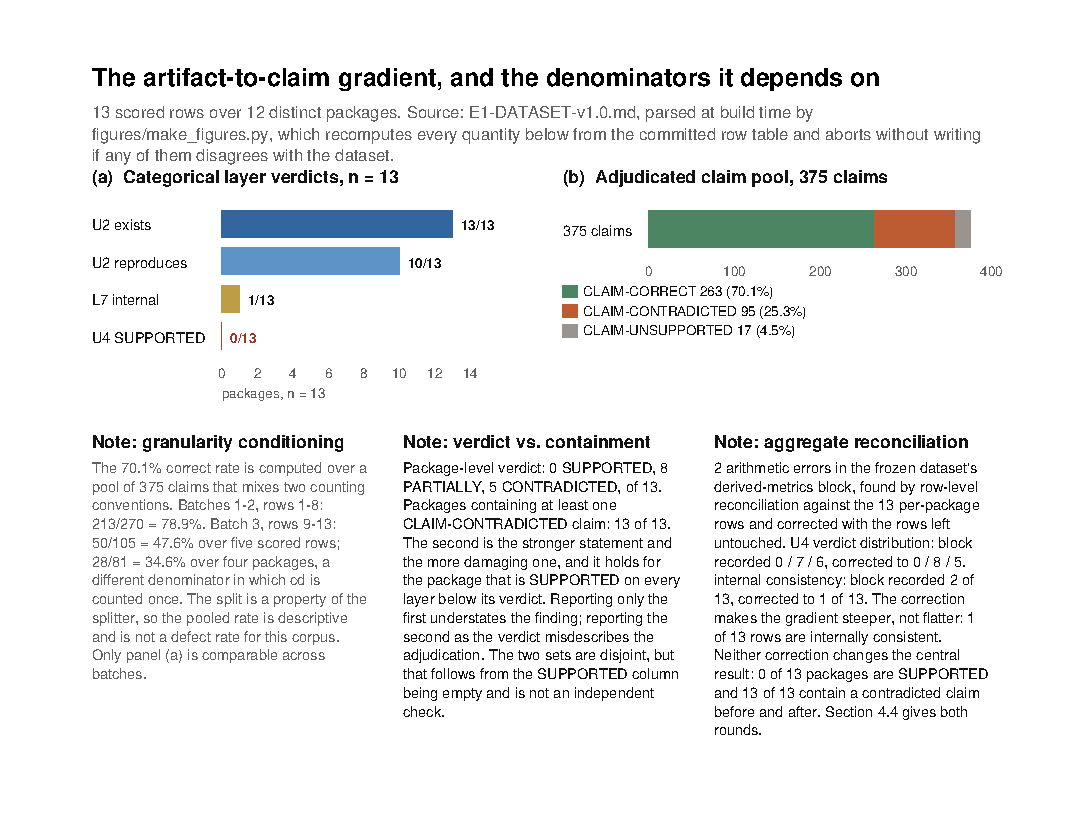
\includegraphics[width=\textwidth]{figures/fig_layer_gradient.pdf}
\caption{The four-layer gradient and the denominators it depends on. (a) The
categorical layer verdicts, denominator 13 and constant across batches. (b)
The adjudicated claim pool, with the two-granularity conditioning stated in
the figure rather than only in the caption. (c) The two package-level
quantities that a reader is most likely to conflate. The note at the foot
records two arithmetic errors found in the dataset's own aggregate layer by
row-level reconciliation, both corrected with the row table left untouched. A
third correction to the same layer --- a layer-label shift carrying no
arithmetic error at all --- postdates this figure and is written up in
Section~\ref{sec:correction}.
Generated by \texttt{figures/make\_figures.py} from
\texttt{figures/data/e1\_rows.csv}.}
\label{fig:gradient}
\end{figure}

\subsection{U1, claim level}
\label{sec:res-claims}

Of 375 adjudicated claims, 263 are correct, 95 are contradicted and 17 are
unsupported. We do not report $70.1\%$ as a defect-complement rate, for the
reason given in Section~\ref{sec:granularity}: the 375 is a pool of two
counting conventions, and the split is $213$ of $270$ at 78.9\% for
batches~1--2 against $28$ of $81$ at 34.6\% for batch~3 over four packages,
or $50$ of $105$ at 47.6\% when batch~3's fifth row is included. The
direction of the split is a property of the splitter.

What the claim-level data does support is a distributional statement that is
insensitive to the convention. The \texttt{UNSUPPORTED} category is 17 claims
in total, spread over eight of thirteen rows, and those are the claims for
which no committed artifact bears on the proposition at all: an ablation table
with no code path that could produce it, four ablation numbers present in no
code and no artifact, a two-word claim about correlation attached to a
quantity the code defines as a single global scalar. A number that is
transcribed correctly from an artifact that does not measure the claimed
quantity is \texttt{CORRECT} at U1 and worthless at U3, and the
\texttt{UNSUPPORTED} column is how the first phenomenon becomes visible.

\subsection{U2, artifact existence and reproduction}
\label{sec:res-repro}

Every one of the thirteen rows ships a committed artifact: 13 of 13. Ten of
thirteen reproduce under auditor execution, and among the reproducing group
the reproduction is frequently exact. Four of the ten regenerate their artifact
byte-identically with no qualification: the covert-detection upstream package
and the audit manuscript's copy of that same artifact, which agree with the
regenerated file by a three-way SHA-256 ---
\texttt{4242d117dff67c716523e694704ca918f2537d47}\allowbreak
\texttt{56cf1d4161938a629c237675} for the regenerated copy, the committed
upstream copy and the audit manuscript's committed copy; the scheduling
package, whose forty-five rows and five fields match exactly; and the co-design
package, whose four policies and eight fields each match exactly. A fifth, the
video-coding package, matches byte-for-byte on every scientific field with a
single wall-clock field differing, which is a measurement of the machine rather
than a result.

Three packages do not regenerate. Two of them diverge because the committed
artifact is valid for one library release and for no other: in both cases the
label count itself differs, so the random stream diverges inside the data
generator rather than in the classifier, and the cause could not be pinned to
a specific release. The third returns a different population size from the one
its own committed results file holds, and that divergence is a code defect
rather than version drift, because the documented contract of the routine is to
return a fixed population and its peeling loop can terminate early.

The pattern that matters is not the count. It is that the three
non-reproducing packages are no worse than the ten reproducing ones at the
layers above, and Section~\ref{sec:res-disagree} quantifies that.

\subsection{U3, the artifact-to-claim relation}
\label{sec:res-relation}

The relation is broken by contradiction in all thirteen rows, which is a
statement about the corpus rather than a finding about any package, because
every row also contains at least one claim that no artifact contradicts. The
substantive U3 result is the second line: in eight of thirteen rows the
relation between some artifact and some claim is \emph{absent} --- the
structure the claim names is not implemented, is implemented and never used,
or is replaced by something else under the same name.

The corpus contains three distinct absence mechanisms, and they are worth
separating because they differ in how easily a reader detects them. In one,
the named structure is constructed and discarded: the state vector, the mixer
Hamiltonian and the variational parameters are each built and each never read,
so the pipeline contains the vocabulary of a variational method and none of its
mechanism. In one, the named structure is replaced rather than omitted: three
published detector names are cited in the bibliography and appear as three
weighted clipped z-scores, with no import of the corresponding libraries
anywhere in the file. In one, the named structure is never built at all, and
the artefact's real subject is a geometry that the manuscript's central
empirical finding is a consequence of.

Absence of this kind is not detectable by any number check, because the
numbers are consistent with the code that exists. It is detectable only by
establishing what the code does against what the text says, which is why U3
is a separate unit and not a corollary of U1.

The frozen record stores the U3 status of each row as a binary, present or
absent, and it does not store which of the three absence mechanisms applies to
which row. We therefore report the count, 8 of 13, and the three mechanisms,
and we do not assert a row-by-row mapping between them, because the dataset
does not contain one.

\textbf{TODO(per-row U3 reason code): a frozen assignment of each
relation-absent row to a specific absence mechanism.} The binary U3 column
records that a relation is absent but not why, and the batch reports
establish the three mechanisms without recording which rows they were observed
in. Resolving this would require re-coding the eight rows against the U3
definition after the fact, which is re-adjudication and would break the freeze
this paper reports against.

\subsection{U4, package verdicts}
\label{sec:res-verdicts}

No package is \texttt{SUPPORTED}. Eight are \texttt{PARTIALLY SUPPORTED} and
five are \texttt{CONTRADICTED}. The dataset's derived-metrics block recorded
seven and six until the row-level reconciliation described in
Section~\ref{sec:correction} corrected it; the block and the row table now
agree, and Table~\ref{tab:recon} records both figures.

The number that is easy to confuse with the verdict distribution is
$13$ of $13$: every package in the corpus contains at least one claim
contradicted by its own artifacts. That is the stronger statement and the more
damning one, and it holds even for the single package that is
\texttt{SUPPORTED} on every layer below its verdict --- the \pkg{cd} audit
manuscript, which holds 22 of 24 claims and whose one contradicted claim is a
standard-deviation estimator disclosure. Reporting the verdict distribution
without the $13$ of $13$ understates the finding. Reporting the $13$ of $13$
as though it were the verdict misdescribes the adjudication. Both appear,
separately, in the dataset and in Figure~\ref{fig:gradient}(c).

A pre-freeze draft of the aggregate summary stated ``12 of 13 packages have
claims contradicted by their own artifacts''. That figure was wrong in both
directions of its construction and is superseded.

\subsection{Cross-layer disagreement}
\label{sec:res-disagree}

The most consequential result in the study is a joint one, and it is
machine-checked. Of the ten rows whose artifact reproduces under auditor
execution, \emph{zero} are \texttt{SUPPORTED}: seven are
\texttt{PARTIALLY SUPPORTED} and three are \texttt{CONTRADICTED}. Of the
three rows that do not reproduce, one is \texttt{PARTIALLY SUPPORTED} and two
are \texttt{CONTRADICTED}, and again none is \texttt{SUPPORTED}. Reproduction
is not a usable proxy for integrity, and in this corpus it is not even
weakly predictive of the verdict: the two groups have the same shape.

The sharpest instance is one package, and it is worth stating precisely
because it is the case a reviewer will ask about. Its committed metrics file
regenerates bit-for-bit across two independent process runs, on every
scientific field, with one wall-clock field differing --- the strongest
reproduction result in the corpus. Its training loop executes a single policy
update at the end of a sixty-thousand-step rollout, where the manuscript
describes per-episode updates over 120 minibatches, so the plotted convergence
curve is the return trajectory of an untrained policy. Its own robustness file
in the same repository reports the method at $-10.26\%$ against its fixed
baseline in stable conditions, with a probability of one of ever winning, and
the manuscript cites neither that file nor any of the ten other robustness
artifacts beside it. Fifteen of its mechanism identities are exactly right and
both of its tables match its artifact in twenty of twenty cells.

The correct characterisation of that package is not that the code is broken.
The trained policy differs measurably from a fresh initialisation, its action
distribution flattens from a mode at $34.1\%$ to a maximum at $18.7\%$, and it
beats a uniform random policy $67.93$ against $62.90$. What is false is the
training procedure the paper describes, the convergence it reports, the
significance evidence it offers, and the central advantage claimed in its
abstract --- and the refutation of that advantage is in the package's own
unreferenced file. A package can be perfectly reproducible and still be wrong,
and reproduction tells you nothing about which.

% ----------------------------------------------------------------------------
% 6. FAILURE TAXONOMY
% ----------------------------------------------------------------------------
\section{Failure Taxonomy}
\label{sec:taxonomy}

The gap decomposes into three classes. We present them as a taxonomy of
relations between computational evidence and scientific assertion, not as a
list of bugs, because each class has a distinct signature in the units of
Section~\ref{sec:model} and a distinct detection requirement.
Figure~\ref{fig:classes} renders the signatures. One further instance of this
taxonomy occurred inside our own apparatus rather than inside a corpus package;
we develop it in Section~\ref{sec:tax-apparatus} and explain there why we
classify it as an instance of the third class rather than as a fourth one.

\begin{figure}[t]
\centering
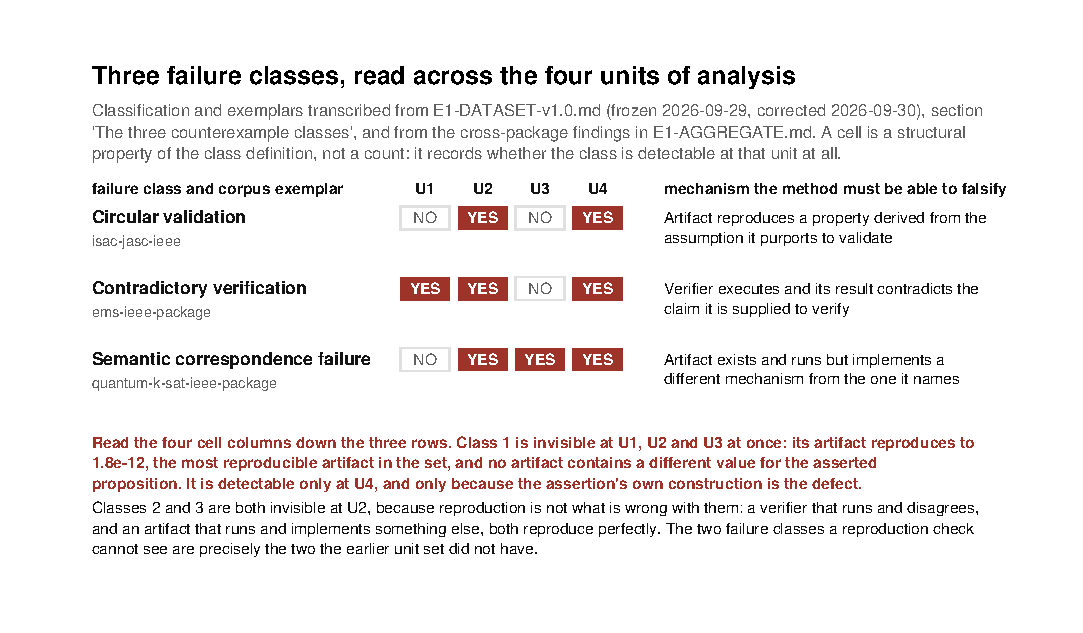
\includegraphics[width=\textwidth]{figures/fig_failure_classes.pdf}
\caption{The three failure classes read across the four units of analysis. A
cell is a structural property of the class definition, not a count: it
records whether the class is detectable at that unit at all. Classification
and exemplars are transcribed from the frozen dataset's counterexample section
and the cross-batch aggregate. Generated by
\texttt{figures/make\_figures.py} from
\texttt{figures/data/failure\_classes.csv}.}
\label{fig:classes}
\end{figure}

\subsection{Circular validation}
\label{sec:tax-circular}

The instrument reproduces the property it is meant to validate. The paradigm
case in the corpus draws its estimator error from the very Cram\'er--Rao
bound it is being tested against, and simultaneously holds the most
reproducible artifact in the set, agreeing to $1.8\times10^{-12}$. It holds
55 of 55 cells of its summary table against its artifact, which is the
cleanest table in the corpus, and its package verdict is
\texttt{CONTRADICTED}.

The mechanism is one line of code and it is not a bug. The simulator
generates samples using a bound that the experiment then compares the
estimator's error against. Agreement is guaranteed by construction, and the
agreement is reported as a validation. Nothing downstream can detect this: the
artifact exists, it reproduces, the number in the paper matches the number in
the file, and the tables agree. The class is detectable only at U4, and only by
an evaluator who asks what the simulation measures rather than whether it
reproduces.

A second instance of the same class appears in the same corpus under a
different name. A mitigation experiment defines two named techniques as
scalar multipliers of a noise parameter --- one as thirty percent less noise,
one as fifty percent less noise --- and then reports that the techniques
improve performance. The figure demonstrates that reducing a parameter
improves a result. It cannot demonstrate that the techniques reduce the
parameter, because the reduction is the definition rather than the finding,
and the paper's mechanistic conclusion, that measurement errors dominate gate
errors, is drawn from the multiplier table and has no support in the code.

\subsection{Contradictory verification}
\label{sec:tax-contradictory}

The artifact is executable and reproducible, and its result contradicts the
claim it is supplied to verify. Three packages in the corpus ship a C
reference kernel that compiles, runs, exits with status zero, and disagrees
with the paper it is bundled with, and in all three the package's own README
instructs the reader to compile and run it. In one the manuscript calls the
file an independent reference kernel in its methods section and in its
readme. The extension of this hazard beyond dead code is the finding: an
unreferenced kernel is a tidiness problem, and a kernel that is advertised as
verification and contradicts the paper is a correctness problem, because a
reviewer who follows the instructions will run three programs that disagree
with the papers, and in one case the disagreement reverses the headline
ranking.

The mechanism is worth naming because it is not accidental. In that case the
C implementation and the Python implementation are two different models: the C
file gives one configuration a pass-through reflector while the Python sets
every element weight to zero, so no reflection at all occurs. The two
codebases cannot serve as mutual checks, and the manuscript offers the C file
as exactly that.

One package in the corpus carries a fourth variant of the same hazard in the
opposite direction, and it is reported for balance. Its kernel is
memory-unsafe and aborts on every run, writing 42 instrumented values into a
41-element buffer, which AddressSanitizer confirms as a heap overflow. That is
a real defect, and the package does not present the kernel as a verification
path: it ships a reduced-configuration test script and labels its own figures
as generated by the simulator. The absence of the advertisement is what keeps
it out of the class above, and it is recorded in the audit as a
negative finding on a suspected defect.

\subsection{Semantic correspondence failure}
\label{sec:tax-semantic}

The artifact exists, can produce results, may even contain structures named
after the claim, and the implemented mechanism does not correspond to the
described one. Four packages in the corpus exhibit it, and the variety is
instructive because the naming is intact in every case.

A package titled as variational optimisation on a noisy basis is a full
classical state-vector simulation in an array library: sixteen thousand
complex amplitudes at the largest instance size, a parameter search that draws
uniform samples and keeps the best, and a noise model that is a
non-norm-preserving coherent admixture of a single basis state, renormalised
away at read-out. Its reported score is the maximum over the ten most
probable bitstrings read at full amplitude precision, presented as
``measurement'', while the classical baseline it is compared against performs
two thousand genuine random flips. The reported gap is therefore between an
oracle and a real search, and the package's own two reported quantities make
the size of the oracle measurable: the reported satisfaction ratio
corresponds to one violated clause, while the circuit's expected number of
violated clauses is more than five.

A second package asserts Pareto optimality in its abstract, its contributions,
its results and its conclusion, and contains no Pareto computation anywhere in
696 lines. It contains an exhaustive enumeration of thirty-two states that
returns exactly one point, minimising a single weighted scalar; a weighted-sum
scalarisation produces a point on a front at best, and no front is ever
computed. It also computes a state vector, a mixer Hamiltonian and four
variational angles, and reads none of them; and its policy machinery executes
to one constant mitigation mask and one constant performance level across all
two hundred steps, so neither of the two components the abstract headlines as
a conjunction influences the executed behaviour. The paper's own tables report
the two halves of that conjunction as interchangeable, and the abstract does
not mention it.

A third package's central empirical finding is that coverage improves as
constellation size increases from ten to three hundred and twenty satellites,
and its own results file shows the relation inverted, with coverage
\emph{falling} as size rises. The measurement that produces the inversion is a
constellation model that does not build the pattern the paper names: twenty
satellites per plane span $21.375^{\circ}$ of arc at $1.125^{\circ}$ spacing,
so the whole three-hundred-and-twenty-satellite design occupies twenty
distinct latitudes inside a band $12.25^{\circ}$ wide. Four coverage
percentages quoted in the results section do not occur anywhere in the
artifact, where the maximum is below sixty per cent. The multi-objective
optimiser itself is correct, deterministic across runs, and its geometry
equations match the code exactly; the defect is in the constellation model,
and the paper's headline follows from it.

A fourth package describes a deep ensemble of three published detectors whose
outputs are fused by learned weights. The three detectors are weighted
clipped z-scores, with no import of any of the corresponding libraries present
in the file; the fusion weights are a hardcoded constant that is never fitted;
the wavelet feature block and the hidden Markov state sequence are both
computed, logged and passed as arguments to a function that ignores them; and
the reinforcement-learning agent, which is called five thousand times, has a
monotone initial action-value table, so its greedy action is the ceiling
threshold from the first step. Its realised action counts over those five
thousand steps run from 1597 selections of the ceiling threshold to 61
selections of the lowest, and the two lowest thresholds together account for
128 of 5000. Two correlation coefficients quoted in its results section are
attributed to a quantity the code defines as a single global average, so they
are not weak, they are structurally incomputable. The package is nonetheless a
well-built one: its committed results file is complete, its results table
reproduces the artifact in twenty of twenty cells, its published negative
result is stated correctly in its own results section, and it is the only
package in the corpus to report that its proposed method underperforms its own
baseline.

The naming is intact in every case in this class, and that is what makes the
class coherent. A correspondence failure is not a missing mechanism; it is a
present vocabulary attached to an absent or different referent. The defect in
this study's own aggregate layer has exactly that shape: every name was intact,
every count was correct, and the referent each name attached to was the wrong
layer. The next subsection treats it.

\subsection{Why the aggregation defect is not a fourth class}
\label{sec:tax-apparatus}

The layer-label shift documented in Section~\ref{sec:correction} is the most
consequential single defect this series produced, it is the cleanest available
demonstration that aggregation integrity is not reducible to internal
arithmetic consistency, and it is tempting to promote it to a fourth entry in
the taxonomy. We have not, and the reason is worth stating because the
taxonomy is the paper's contribution and the temptation points at the paper's
own thesis.

The aggregate asserted that a layer named \texttt{L6} measured internal
consistency when the rubric and the primary records call that layer
\texttt{L7}. The counts were all correct; the meaning was not. That is the
definition of the third class, applied at a different location in the chain:
an artifact exists, is derived from records that reproduce, and implements a
different referent from the one it names. The class is defined by a structural
relation between a name and a referent, not by where in the chain the name
lives, and on that definition the aggregate instance is a subtype of semantic
correspondence failure rather than a sibling of it. Promoting a subtype to a
sibling is the step at which a taxonomy becomes a list, and three reasons
concrete to this study make the promotion actively wrong.

First, provenance. The three classes are transcribed from the frozen dataset
of record, and each has an exemplar with a committed artifact behind it. The
aggregate defect has no exemplar in that sense: it was found in the
instrument, not in a corpus package, and asserting it as a peer class would
require a definition the frozen record does not contain. Second, scope. This
paper claims the three classes are exhaustive over the thirteen rows in which
they were found, and Section~\ref{sec:threat-domain} states that scope
explicitly. The fourth instance was not found in the thirteen rows, so
extending the taxonomy would silently widen the claim from a corpus finding to
a general one --- which is precisely the extrapolation rule R5 exists to
forbid. Third, and decisively for a taxonomy whose stated value is that each
class carries a distinct detection requirement: the label shift does not
require a new kind of check. It requires the same check the third class
already demands, applied one level up --- establish what the code does against
what the text says, and here, what the summary does against what the instrument
defines. Two checks differing in where they are pointed is one method.

What the instance does earn is a place in the argument rather than in the
taxonomy, and we give it one. It is the only case in this series in which
correspondence failed inside the evaluation apparatus while arithmetic held
perfectly, which makes it the sharpest available answer to the objection that
a taxonomy of relation failures is a distinction without a difference. The
apparatus is not exempt from the apparatus's own rubric.

% ----------------------------------------------------------------------------
% 7. CASE STUDIES
% ----------------------------------------------------------------------------
\section{Case Studies}
\label{sec:cases}

The cases are chosen to make the taxonomy concrete and to answer the obvious
objection to a corpus of negative findings. Each is drawn from the batch
report that measured it.

\subsection{\pkg{isac}: circular validation with the best reproduction in the set}
\label{sec:case-isac}

This is the paradigm case of Section~\ref{sec:tax-circular} and it is worth
the detail because it isolates the failure from every ordinary explanation.
The package holds 81 adjudicated claims, 70 of them correct, 11 contradicted
and none unsupported. Its artifact regenerates to $1.8\times10^{-12}$, the
most exact agreement in the corpus, and 55 of 55 cells of its summary table
agree with the artifact across five metrics by eleven signal-to-noise points.
Its abstract's only headline number is refuted by the paper's own table. Its
claim that the standard error exceeds four units across the range is
contradicted by a sweep whose maximum is under three; its claim that the
velocity spread stays below five metres per second is violated at nine of
eleven points, reaching more than a hundred at the lowest signal level; and
nine cells of its README table are wrong by up to a factor of thirty-three.

None of that is the interesting part. The interesting part is that the
defect --- estimator error drawn from the very bound it is tested against ---
is invisible to every measurement reported, and that the reproduction quality
which makes the package look best-built in the corpus is orthogonal to it.
Good simulation hygiene buys nothing when the defect lives in what the
simulation measures.

\subsection{\pkg{ems}: a verifier that reverses the conclusion}
\label{sec:case-ems}

This is the paradigm case of Section~\ref{sec:tax-contradictory}. The package
holds 18 adjudicated claims, 12 correct, 3 contradicted and 3 unsupported. All
sixteen cells of its results table match the committed artifact to three
significant figures, and the artifact regenerates bit-for-bit on every
quantity the paper reports, on a toolchain far newer than the artifact's.
Both headline values, and the security metric the abstract leads with, are
correct. The Monte Carlo robustness claim --- that no realisation falls below
minus ten decibels --- is measurably true, at zero of one hundred, with a
minimum of $-3.96$~dB, and it survived an auditor prediction that it would
fail. Seven of its eight figures have committed generators that ran.

The package ships a 245-line C file that the methods section calls an
independent reference kernel and the README instructs the reader to compile
and run. It compiles, it runs, it exits zero, and it disagrees with the paper
on three of four configurations. On one it differs by $11.55$~dB with the
\emph{opposite sign}, which reverses the paper's central ranking: the kernel
makes the pass-through configuration the best, where the paper's headline is
that the steered configuration wins. The cause is that the two files implement
different models, so the C file cannot serve as the check it is offered as.

The remaining defects are of the correspondence kind rather than the numerical
kind, and they are worse for the paper's conclusion even though they change
no number. The beam is steered at a hardcoded default angle that misdirects it
by more than twenty degrees from the receiver, forfeiting nearly fifteen
decibels of available gain. The ``complete suppression'' at the eavesdropper
credited as the fundamental mechanism of the security improvement is a
magnitude below the float64 cancellation floor for a sum of that many
unit-magnitude terms, so the suppression is floating-point noise rather than
physics. The stated shadow-fading standard deviation is twice the implemented
one, and the surviving Monte Carlo robustness claim holds only because of that
error: at the implemented value the probability of any realisation breaching
the stated threshold is zero, and at the paper's stated value it is over
half. One figure has no generator at all and its eight panels are identically
zero, and it survives re-execution only because nothing writes it.

\subsection{\pkg{quantum-k-sat}, \pkg{qce}, \pkg{mega-constellation}, \pkg{icft}}
\label{sec:case-semantic}

The four correspondence cases are developed in
Section~\ref{sec:tax-semantic}. Their claim splits are $25/13/11/1$,
$18/11/5/2$, $16/6/6/4$ and $25/11/13/1$ for total, correct, contradicted and
unsupported respectively. Two of the four hold the only clean figure layer and
the best transcription fidelity in their batch, and one of the four is the
corpus's most methodologically careful package on the layer that matters.

Three further points are worth recording because they bear on the taxonomy
rather than on the individual packages. First, in one of them the
significance test reported is impossible: the two arms are generated in
separate loops and run on different instances, so a paired test has nothing
to pair, and the per-trial data needed to run any test is not committed at
all. The effect size the paper reports is internally consistent with the
paper's own dispersion figures and externally inconsistent with the artifact,
which yields a materially larger value. Second, in another, a headline
percentage is arithmetically correct on an uncontrolled comparison: the three
arms of the experiment each receive a different draw of the hardware noise
parameters because the generator's random stream is advanced between them and
never reset, and the arm that wins received the best draw. Holding the
hardware draw fixed across arms --- an experiment the auditor wrote and ran ---
roughly halves the effect, and the effect survives. The right finding there is
not that the result is fabricated but that it is the correct arithmetic on a
comparison against a moving baseline. Third, in a fourth, the crossover
operator does not enforce the declared decision-variable bounds while the
mutation operator does, which is measurable over twenty thousand crossovers:
$110$ offspring fall outside the declared altitude range. The auditor's
first version of that test used two identical parents, which makes the
operator a no-op and returned zero violations; the test was discarded and
re-run, and the corrected test is the one reported.

\subsection{\pkg{cd} as a near-positive case}
\label{sec:case-cd}

This case answers the objection that a corpus of failures proves nothing but
the selection of the corpus, and it is the control the method needs.

The \pkg{cd} programme contains two artifacts. The upstream package's
artifact regenerates byte-for-byte, confirmed by a three-way hash agreement
between the regenerated file, the committed upstream file and a third
committed copy --- the strongest single reproduction result in the corpus.
The audit manuscript written about that package holds 22 of 24 adjudicated
claims, is supported on every layer below its internal-consistency layer,
presents an unusually candid limitations section that flags its own novelty
risk and declines to correct for a ceiling effect, and is the only manuscript
in the corpus that is largely supported on its own evidence. Its central
selection finding is the strongest in the corpus: one detector's metric is
pinned at its ceiling with exactly zero dispersion across all twenty seeds, so
no significance test on that column can return a p-value, and the per-seed
difference between the two leading detectors is exactly zero in seventeen of
twenty trials, which makes the ranking the paper reports unrecoverable. It
reports that, and it explicitly declines to select a harder operating point
and re-run, on the stated grounds that doing so would change the experiment
rather than audit it.

And it still contains a detectable artifact-to-claim contradiction. Its table
declares that it reports the sample standard deviation on $n-1$. Its own
committed statistics file carries both estimators. The printed values are the
population ones: for the autoencoder the population value rounds to the
printed four decimals and the sample value does not, and the same holds for
two of the other four detectors. The difference is under $0.001$ on every
cell and it changes no conclusion. It is a claim about method, it is
falsifiable from the paper's own artifact, and it is false.

That is the calibration the method needs. A five-figure package with a
five-figure ledger, a bit-reproducible artifact, a hash agreement established
three independent ways and twenty-two of twenty-four claims holding still
carries a detectable artifact-to-claim contradiction. The defect is not a
symptom of sloppiness at scale, and no threshold of build quality separates
the packages that carry one from the packages that do not.

The upstream package is a different object and a different verdict. Its
artifact also regenerates bit-for-bit, and its manuscript holds 3 correct, 17
contradicted and 1 unsupported claim of 21 adjudicated. Both of its stated
conclusions are contradicted by its own artifact. Same research programme, two
artifacts, two verdicts, and the earlier rubric's single
\texttt{PARTIALLY SUPPORTED} for the pair was the rubric's defect.

% ----------------------------------------------------------------------------
% 8. THREATS TO VALIDITY
% ----------------------------------------------------------------------------
\section{Threats to Validity}
\label{sec:threats}

\subsection{Author-controlled corpus}
\label{sec:threat-corpus}

The corpus was authored primarily by the first author, who had direct
knowledge of the implementation history and publication context of every
package. Every bias that threatens an author-controlled corpus applies here,
and the controls of Section~\ref{sec:method-bias} reduce but do not remove
them. Specifically: the choice of which packages to include was not random and
was made by the author; the claim enumeration reflects the author's reading of
what each manuscript asserts; and an author who knows that a package contains
a defect is more likely to find it, which inflates the contradiction rate
relative to a blind audit even when the adjudication is frozen and the
negative findings are retained without exception.

The same fact is what makes the mechanism results possible. Distinguishing an
artifact that is badly designed from one designed to mislead requires
knowledge of intent that a third-party auditor does not have. The weakness and
the strength are the same fact, and we state both rather than choosing the
flattering one. Nothing in this paper is a prevalence estimate, and no
percentage here should be read as describing packages outside the audited
rows.

\subsection{Corpus size, and why no inference is licensed}
\label{sec:threat-n}

The corpus is thirteen scored rows over twelve distinct packages, drawn from
one author. The absence of any inferential claim here is not a statistical
power shortfall awaiting more data, and we do not frame it as one. There is no
power problem to remedy, because the corpus was not constructed as a
probabilistic sample of any defined population. It is the set of thirteen
research packages that exist and that were selected because they were
auditable. No population was defined, no sampling frame exists, and no
randomisation occurred. An interval estimate, a significance test or an effect
size would each presuppose a sampling model in which these thirteen rows are
realisations of a random draw from a superpopulation, and this study has no
such model and cannot acquire one by auditing more packages under the same
design. A fourteenth row would be a fourteenth adjudicated case, not a
fourteenth draw. The correct statement is that \emph{no amount of additional
data from this design would license this inference}.

Two distinct things follow, and conflating them is how a design limitation
comes to be misreported as a data limitation. The first is that no
inferential claim is made, because the design does not license one; that is a
property of the design and is not contingent on how much data the design
produces. The second is that the two headline figures have margin on grounds
that have nothing to do with sampling. $13$ of $13$ and $0$ of $13$ are
saturated counts: the first is a tally over the audited set and the second is
the rubric's own verdict rule applied to every row, so no plausible
reclassification moves either. The intermediate counts --- ten of thirteen
reproducing, one of thirteen internally consistent, eight of thirteen with an
absent relation --- are likewise exact tallies of the frozen rows. They are
reported descriptively, they carry no sampling error, and they should not be
read as estimates of anything. A reclassification moves them by construction
rather than by sampling, which is a different objection and the one
Section~\ref{sec:correction} answers.

That the intermediate counts are the fragile ones is not hypothetical here:
they are exactly the counts the aggregation layer got wrong, on more than one
occasion, and on a third occasion the defect lay in the names attached to
those counts rather than in the counts themselves. This is why the correction
log of Section~\ref{sec:correction} treats a reconciliation step as part of
the method rather than as a final proofread, and why reconciling against the
rows is not on its own a sufficient check on a summary layer.

\subsection{Mixed claim granularity}
\label{sec:threat-gran}

The claim-level figures pool two counting conventions, as
Section~\ref{sec:granularity} states. The pooled $375$ and the $70.1\%$ derived
from it are descriptive, and the split between batches --- $78.9\%$ against
$34.6\%$ --- is a property of the convention rather than of the packages. The
categorical layer and package verdicts do not depend on granularity and are
the results this paper rests on. A second corpus scored under a fixed
granularity is required before any claim-level rate from this line of work
should be compared with anything.

\textbf{TODO(single-granularity re-adjudication): the total claim count and
the correct rate at one fixed claim granularity across all thirteen rows.} A
single frozen granularity would require re-adjudicating all thirteen rows
under the rubric's U1 definition and re-freezing the dataset, which is a new
corpus version rather than a correction to this one, and which cannot be
performed without breaking the freeze this paper reports against.

\subsection{Domain heterogeneity}
\label{sec:threat-domain}

The thirteen packages span radio propagation, covert detection, deep
reinforcement learning for video coding, electromagnetic eavesdropping
immunity, combinatorial optimisation for satellite constellations, market
manipulation detection, event-driven scheduling, and quantum-inspired
combinatorial search. There is no shared benchmark, no shared metric and no
shared task. The taxonomy of Section~\ref{sec:taxonomy} is therefore a
taxonomy of the artifact-to-claim \emph{relation}, not of any scientific
domain, and its three classes are claimed to be exhaustive only over the
thirteen rows in which they were found.

\subsection{Reproduction environment}
\label{sec:threat-env}

Every reproduction was performed on a single machine with a single toolchain
family, newer than the one the artifacts were committed under. That cuts both
ways and both directions are reported. It makes the reproduction results
conservative in one sense, because a newer library is more likely to break an
old artifact than an older one would, and the two non-reproducing packages
whose cause is a library-scope effect were found this way. It also means the
ten reproducing rows are reproduced on one toolchain and not on several, so
this paper cannot distinguish a genuinely platform-independent artifact from
one that happens to survive one toolchain. The one package for which a
wall-clock field differs is reported as a hardware difference rather than a
result difference, and that call is a judgement.

\subsection{Rubric dependence}
\label{sec:threat-rubric}

Every number in this paper is a function of a rubric, and a different rubric
would produce a different set. The corpus is small enough that the
package-verdict column is not robust to the rubric's verdict text: one
package's verdict changed during this series, from \texttt{PARTIALLY
SUPPORTED} to \texttt{CONTRADICTED}, on a mechanical application of the same
rubric's own criterion to a different layer of the same research programme,
and a second package's layer~2 verdict was overturned by an evaluator who
declined to accept the rubric's own premise. Both changes are recorded in the
dataset rather than absorbed, and the rubric was corrected to score the two
artifacts of that programme separately. A reader who rejects the rubric's
verdict text should expect the intermediate counts of
Table~\ref{tab:metrics} to move. The two headline figures should not.

There is no inter-rater reliability statistic anywhere in this series. Each
batch was adjudicated by a single evaluator, batch~1 by a delegated agent and
batches~2 and~3 by separate agents, and no row was independently
double-coded.

\textbf{TODO(inter-rater reliability): an agreement coefficient over the
twelve units of the four-unit scheme.} A second independent adjudicator would
have to re-score a sample of rows from the artifacts without access to the
first adjudicator's findings, and the resulting statistic does not exist in
the frozen record and cannot be reconstructed from it.

\subsection{Novelty has not been assessed}
\label{sec:threat-novelty}

This manuscript cites no prior work, and that is a deliberate choice rather
than an oversight: inventing references to satisfy a citation requirement would
be a worse defect than the absence, and the two earlier papers in this series
made the same choice and stated the same risk. The consequence is real and we
state it plainly. No novelty assessment against prior work in
reproducibility methodology, artifact evaluation, or research software
engineering has been performed. We do not know whether a four-unit
claim/artifact/relation/package decomposition with a frozen verdict vocabulary
has been proposed before, whether the three failure classes have been named,
or whether the same result has been reported on a different corpus. A reviewer
should treat the novelty of the contribution as open, and the authors accept
that a reviewer who performs the search we did not may find prior art.
Section~\ref{sec:intro-scope} states this as a first-class limitation in the
introduction rather than leaving it to this subsection alone.

\textbf{TODO(novelty assessment): a positioning review against published work
on artifact evaluation and reproducibility measurement.} This requires a
literature search, an inclusion criterion and a comparison table against
prior taxonomies of artifact-to-claim failure. Neither this manuscript nor the
two earlier papers in the series has a reference list, so no such comparison
exists anywhere in the material available to us.

% ----------------------------------------------------------------------------
% 9. DISCUSSION
% ----------------------------------------------------------------------------
\section{Discussion}
\label{sec:discussion}

\subsection{Reproducibility versus integrity}
\label{sec:disc-repro}

The empirical claim of this paper is narrow and we state it as a claim about
thirteen rows: reproducibility and artifact-to-claim integrity are
independent properties in this corpus, and the second is the one a reader
depends on. Ten of thirteen artifacts reproduce and zero of thirteen packages
are fully supported, and the joint distribution shows no relationship between
the two. The mechanism behind the independence is not mysterious. Reproduction
tests whether the code does what the code does. Integrity tests whether the
code does what the paper says. These coincide only when the paper describes
the code accurately, and the frequency with which they coincide is an empirical
question about writing, not about software.

The practical implication is that a reproducibility result should not be
reported as an integrity result, and an integrity result should not be
compressed into a reproduction statistic. The most common compression we found
in practice --- including in our own dataset's first draft --- is to quote a
claim-level percentage without the granularity that produced it, and to quote a
package-level verdict without noting that a single contradicted claim is
sufficient to move a package off \texttt{SUPPORTED}.

\subsection{Verifiers as evidence}
\label{sec:disc-verifiers}

The second discussion point is about the semantics of a verification artifact.
Three packages in the corpus ship a C file described as an independent
reference implementation, presented as corroboration, which disagrees with the
paper when run. The general point is that a reference implementation is not
evidence unless it is derived independently of the implementation it checks
and unless its agreement is established by running both. In all three packages
the C file is derived from the same understanding of the model as the Python
file, so agreement between them is not independent confirmation of anything,
and disagreement between them is evidence that one of them does not implement
the paper. Either way the advertisement is wrong, and in one case it is wrong
in a way that reverses a headline result.

The correct handling is cheap. A reference implementation that is wired into
the test suite, that fails the build when it disagrees, and that is regenerated
by the same command as the main artifact, is worth more than a paragraph
describing it. A reference implementation that a reader is invited to run by
hand, and that nobody has run, is a liability with a README attached.

\subsection{The danger of executable disagreement}
\label{sec:disc-danger}

A verifier that runs and disagrees is worse than no verifier, because it
transfers false confidence. The reader's update is not ``this package's claim
is wrong''; it is ``this package was checked''. Where the check is a
paragraph of prose describing an independent implementation, and the
implementation is a file nobody compiles, the reader receives the confidence
without the check, and the package's own language supplies the warrant.

We think this is the most transferable finding in the study, and it is
transferable precisely because it is not about a domain. Any artifact that
advertises a verification path has an obligation to establish that the
verification passes. In the corpus, three packages ship a C kernel that their
README instructs the reader to compile and run as a check, and all three
disagree with their own paper when run. One of the three does agree with its
paper on one published table --- the optimiser's policy table, which the
kernel reproduces exactly --- while reporting a perfect reliability score
against the paper's headline figure. Partial agreement from an unexecuted
verifier is the worst case, because it licenses exactly the inference the
verification was supposed to prevent.

\subsection{Implications for artifact evaluation}
\label{sec:disc-impl}

Three implications follow for anyone building or applying an artifact
evaluation instrument.

First, fix the unit of analysis before adjudication begins, in the rubric
rather than in the evaluator's head. Our own corpus demonstrates the cost of
leaving it implicit: the first pooled figure was wrong by a factor of 1.19 in
the denominator and by 12.9 points in the numerator, and the two granularities
are still pooled in the frozen record because the freeze forbids re-adjudication.

Second, separate the unsupported status from the contradicted status and never
merge them in a single column. A claim with no artifact and a claim with a
contradicting artifact are in different epistemic positions, and a merged
column makes a package look better evidenced than it is.

Third, add a relation unit, and require at least one relation verdict per
named mechanism. The three classes in Section~\ref{sec:taxonomy} were all
found by asking what the code does, not by asking whether the numbers agree,
and two of the three are undetectable at every other unit. An evaluation
instrument without a relation unit will pass all three.

What survived is the other half of the recommendation, and we state it as
plainly as the failures. Section~\ref{sec:survived} records what held.

% ----------------------------------------------------------------------------
% WHAT SURVIVED
% ----------------------------------------------------------------------------
% Unnumbered so that the numbered structure of the paper is exactly the ten
% sections of the plan, with What Survived sitting between Discussion and
% Conclusion. Same device as the correction notice in the companion paper.
\section*{What Survived}
\addcontentsline{toc}{section}{What Survived}
\label{sec:survived}

An audit that only finds faults is not a balanced audit, and the confirmed
results are what make the negative ones defensible. Rule R7 of the rubric
requires this section, and it is a required part of the method rather than a
courtesy.

\begin{table}[t]
\centering
\caption{Recorded results that survived adjudication. These are the findings
that make the negative results credible: each is a claim the audited package
got right, confirmed by re-execution rather than by reading.}
\label{tab:survived}
\small
\setlength{\tabcolsep}{3.4pt}
\begin{tabular}{>{\raggedright\arraybackslash}p{0.235\columnwidth}>{\raggedright\arraybackslash}p{0.46\columnwidth}}
\toprule
Package & Surviving result \\
\midrule
\pkb{isac} & 55 of 55 cells of the summary table agree with the artifact. \\
\pkb{camae} & All 36 table cells and 45 of 45 summary cells exact. \\
\pkb{sc} & All 24 table cells and the adaptive-selection result hold. \\
\pkb{ems} & All 16 cells of the main table; the Monte Carlo claim survived a prediction that it would fail, at 0 of 100 below $-10$~dB, minimum $-3.96$~dB. \\
\pkb{qce} & The published policy table was confirmed by \emph{executing} the optimiser, not by reading it. \\
\pkb{quantum-k-sat} & All four figures have committed generators that ran; 13 of 14 transcribed numbers correct; no seed or best-case selection. \\
\pkb{sra} & The results artifact regenerates bit-for-bit, 45 of 45 rows; zero unsupported claims; the makespan null result is disclosed in the manuscript. \\
\pkb{mega-const.} & The multi-objective optimiser is a correct deterministic implementation, two runs byte-identical; four of five system-model equations match to the digit. \\
\pkb{h266} & Regenerates bit-for-bit across two fresh processes; fifteen mechanism identities exactly right; the trained policy beats a uniform random policy $67.93$ against $62.90$ and its action mode flattens from $34.1\%$ to $18.7\%$. \\
\pkb{icft} & Committed results file complete; results table reproduces 20 of 20 cells; its own negative result published in its results section. \\
\pkb{cd} audit & Regenerates byte-for-bit by three-way hash; 22 of 24 claims hold; the strongest selection analysis in the corpus. \\
\bottomrule
\end{tabular}
\end{table}

Three of these deserve comment because they cut against the paper's own
interest. The reinforcement-learning policy in one package genuinely works:
it beats a uniform random policy by more than five units of its own quality
metric, and its action distribution measurably flattens under training. The
package's failure is the training loop its manuscript describes and the
robustness study it does not read, not the method. The multi-objective
optimiser in another package is a correct, deterministic implementation, and
four of its five system-model equations match the code to the digit; its
failure is a constellation model that does not build the pattern the paper
names. And a third package published its own negative result, stating in its
results section that its proposed method achieves a lower score than its own
baseline, and repeated it in its limitations. That is the opposite of the
defect pattern the rest of the corpus exhibits, and it is why the package is
\texttt{CONTRADICTED} rather than worthless: the author knew the headline was
bad and published it anyway.

% ----------------------------------------------------------------------------
% 10. CONCLUSION
% ----------------------------------------------------------------------------
\section{Conclusion}
\label{sec:conclusion}

Correct numerical output is not sufficient evidence of artifact-to-claim
integrity, and the separation is not a matter of degree. In a frozen corpus
of thirteen scored rows, ten artifacts reproduce under auditor execution and
zero packages are fully supported; every package in the corpus contains at
least one claim contradicted by its own artifacts; and the reproduced group
and the supported group are disjoint, which the committed figure script
verifies mechanically on every run. The claim-level pool of 375 adjudicated
claims, of which 263 hold, is reported as descriptive and is conditioned by
two counting conventions, and it is not the result this paper rests on.

The gap decomposes into three classes that a reproduction check cannot detect
and a number check cannot detect either: circular validation, in which the
artifact reproduces a property derived from the assumption it purports to
validate; contradictory verification, in which a supplied verifier runs and
disagrees; and semantic correspondence failure, in which an artifact runs and
implements a different mechanism from the one it names. Each was found by
asking what the code does, not by asking whether the numbers agree, and each
lives in the relation between an artifact and a claim, which is the unit an
earlier layer rubric did not have.

The methodological results are the negative ones about our own instrument. The
dataset's aggregate layer failed its own consistency check four times, in three
entries of the dataset's correction log. The first three were arithmetic, and
all three were found by one procedure: sum the thirteen per-package rows, then
compare the sum against the summary block. The first was caught before the
freeze and corrected before any figure was cited. The second and third were
found after the freeze, by the reconciliation this paper runs against its own
data, and are logged rather than quietly amended: a verdict distribution
recorded as $0 / 7 / 6$ where the rows give $0 / 8 / 5$, and an
internal-consistency count recorded as $2$ of $13$ where the recorded column
gives $1$ of $13$. In all three cases the thirteen rows were correct and the
summary was not.

The fourth was not arithmetic, and it is the one that constrains the method.
The aggregate's headline table carried its layer labels shifted by one from L3
upward against the frozen rubric and against all three batch reports, so that
a correct count of $6$ of $13$ was attached to L3 --- Figure where the rubric
calls it L4. Every count reconciled; only the names moved. Because the
aggregate file was already public, that correction is post-publication. It was
found not by reconciliation but by parsing the label sequence and asserting it
against the rubric, and that assertion now runs in this manuscript's
verification script. Eight evaluator self-corrections are in the record,
including an evaluator who overturned the rubric's own premise, an evaluator
who declined to inherit five numbers that appear in no committed artifact, and
an evaluator who caught an off-by-one that would have published a false
contradiction against the rubric's own reference case. The aggregation layer
requires the same audit as the artifacts, and a dataset that fails its own
consistency check is the same failure class this paper describes, one level up.
We report that failure four times over rather than once because two of the
corrections move the reported gradient in the direction that weakens our own
claim, and correcting them anyway is the only version of the gradient that is
citable --- and because the fourth shows that the arithmetic check which caught
the first three is not sufficient on its own. A summary layer must be checked
against the instrument it summarises, not only against itself.

Four limitations are load-bearing and are stated as such. The corpus is
author-controlled, which is a weakness for any prevalence claim and the only
way to attribute mechanism. The corpus is thirteen rows and is not a
probability sample of any defined population, so no interval estimate is
offered --- not because thirteen rows are too few to support one, but because
the design licenses none and more rows of the same kind would not change that;
the two saturated counts the paper rests on do not depend on the argument.
The claim-level figures pool
two granularities and are not comparable to any single-batch figure. And no
novelty assessment against prior work in reproducibility methodology has been
performed, because neither this manuscript nor the two earlier papers in the
series has a reference list; a reviewer who searches where we did not may find
prior art, and we accept that outcome rather than conceal the gap by inventing
citations.

The immediate next step is a second corpus scored under a single frozen claim
granularity, with independent double-coding on a sample, which is what would
convert the categorical gradient reported here into a claim-level rate that
could be compared with anything.

\end{document}
